\documentclass[]{article}
    %%%%%%%%%%%%%%%%%%%%%%%%%%%%%%%%%%%%%%%%%
% Lachaise Assignment
% Structure Specification File
% Version 1.0 (26/6/2018)
%
% This template originates from:
% http://www.LaTeXTemplates.com
%
% Authors:
% Marion Lachaise & François Févotte
% Vel (vel@LaTeXTemplates.com)
%
% License:
% CC BY-NC-SA 3.0 (http://creativecommons.org/licenses/by-nc-sa/3.0/)
% 
%%%%%%%%%%%%%%%%%%%%%%%%%%%%%%%%%%%%%%%%%

%----------------------------------------------------------------------------------------
%	PACKAGES AND OTHER DOCUMENT CONFIGURATIONS
%----------------------------------------------------------------------------------------

\usepackage{amsmath,amsfonts,stmaryrd,amssymb} % Math packages

\usepackage{enumerate} % Custom item numbers for enumerations

\usepackage[ruled]{algorithm2e} % Algorithms

\usepackage[framemethod=tikz]{mdframed} % Allows defining custom boxed/framed environments

\usepackage{listings} % File listings, with syntax highlighting
\lstset{
	basicstyle=\ttfamily, % Typeset listings in monospace font
}

%----------------------------------------------------------------------------------------
%	DOCUMENT MARGINS
%----------------------------------------------------------------------------------------

\usepackage{geometry} % Required for adjusting page dimensions and margins

\geometry{
	paper=a4paper, % Paper size, change to letterpaper for US letter size
	top=2.5cm, % Top margin
	bottom=3cm, % Bottom margin
	left=2.5cm, % Left margin
	right=2.5cm, % Right margin
	headheight=14pt, % Header height
	footskip=1.5cm, % Space from the bottom margin to the baseline of the footer
	headsep=1.2cm, % Space from the top margin to the baseline of the header
	% showframe, % Uncomment to show how the type block is set on the page
}

%----------------------------------------------------------------------------------------
%	FONTS
%----------------------------------------------------------------------------------------

\usepackage[utf8]{inputenc} % Required for inputting international characters
\usepackage[T1]{fontenc} % Output font encoding for international characters

% \usepackage{XCharter} % Use the XCharter fonts\usepackage{XCharter} % Use the XCharter fonts

%----------------------------------------------------------------------------------------
%	COMMAND LINE ENVIRONMENT
%----------------------------------------------------------------------------------------

% Usage:
% \begin{commandline}
%	\begin{verbatim}
%		$ ls
%		
%		Applications	Desktop	...
%	\end{verbatim}
% \end{commandline}

\mdfdefinestyle{commandline}{
	leftmargin=10pt,
	rightmargin=10pt,
	innerleftmargin=15pt,
	middlelinecolor=black!50!white,
	middlelinewidth=2pt,
	frametitlerule=false,
	backgroundcolor=black!5!white,
	frametitle={Command Line},
	frametitlefont={\normalfont\sffamily\color{white}\hspace{-1em}},
	frametitlebackgroundcolor=black!50!white,
	nobreak,
}

% Define a custom environment for command-line snapshots
\newenvironment{commandline}{
	\medskip
	\begin{mdframed}[style=commandline]
}{
	\end{mdframed}
	\medskip
}

%----------------------------------------------------------------------------------------
%	FILE CONTENTS ENVIRONMENT
%----------------------------------------------------------------------------------------

% Usage:
% \begin{file}[optional filename, defaults to "File"]
%	File contents, for example, with a listings environment
% \end{file}

\mdfdefinestyle{file}{
	innertopmargin=1.6\baselineskip,
	innerbottommargin=0.8\baselineskip,
	topline=false, bottomline=false,
	leftline=false, rightline=false,
	leftmargin=1cm,
	rightmargin=1cm,
	singleextra={%
		\draw[fill=black!10!white](P)++(0,-1.2em)rectangle(P-|O);
		\node[anchor=north west]
		at(P-|O){\ttfamily\mdfilename};
		%
		\def\l{3em}
		\draw(O-|P)++(-\l,0)--++(\l,\l)--(P)--(P-|O)--(O)--cycle;
		\draw(O-|P)++(-\l,0)--++(0,\l)--++(\l,0);
	},
	nobreak,
}

% Define a custom environment for file contents
\newenvironment{file}[1][File]{ % Set the default filename to "File"
	\medskip
	\newcommand{\mdfilename}{#1}
	\begin{mdframed}[style=file]
}{
	\end{mdframed}
	\medskip
}

%----------------------------------------------------------------------------------------
%	NUMBERED QUESTIONS ENVIRONMENT
%----------------------------------------------------------------------------------------

% Usage:
% \begin{question}[optional title]
%	Question contents
% \end{question}

\mdfdefinestyle{question}{
	innertopmargin=1.2\baselineskip,
	innerbottommargin=0.8\baselineskip,
	roundcorner=5pt,
	nobreak,
	singleextra={%
		\draw(P-|O)node[xshift=1em,anchor=west,fill=white,draw,rounded corners=5pt]{%
		Question \theQuestion\questionTitle};
	},
}

\newcounter{Question} % Stores the current question number that gets iterated with each new question

% Define a custom environment for numbered questions
\newenvironment{question}[1][\unskip]{
	\bigskip
	\stepcounter{Question}
	\newcommand{\questionTitle}{~#1}
	\begin{mdframed}[style=question]
}{
	\end{mdframed}
	\medskip
}

%----------------------------------------------------------------------------------------
%	WARNING TEXT ENVIRONMENT
%----------------------------------------------------------------------------------------

% Usage:
% \begin{warn}[optional title, defaults to "Warning:"]
%	Contents
% \end{warn}

\mdfdefinestyle{warning}{
	topline=false, bottomline=false,
	leftline=false, rightline=false,
	nobreak,
	singleextra={%
		\draw(P-|O)++(-0.5em,0)node(tmp1){};
		\draw(P-|O)++(0.5em,0)node(tmp2){};
		\fill[black,rotate around={45:(P-|O)}](tmp1)rectangle(tmp2);
		\node at(P-|O){\color{white}\scriptsize\bf !};
		\draw[very thick](P-|O)++(0,-1em)--(O);%--(O-|P);
	}
}

% Define a custom environment for warning text
\newenvironment{warn}[1][Warning:]{ % Set the default warning to "Warning:"
	\medskip
	\begin{mdframed}[style=warning]
		\noindent{\textbf{#1}}
}{
	\end{mdframed}
}

%----------------------------------------------------------------------------------------
%	INFORMATION ENVIRONMENT
%----------------------------------------------------------------------------------------

% Usage:
% \begin{info}[optional title, defaults to "Info:"]
% 	contents
% 	\end{info}

\mdfdefinestyle{info}{%
	topline=false, bottomline=false,
	leftline=false, rightline=false,
	nobreak,
	singleextra={%
		\fill[black](P-|O)circle[radius=0.4em];
		\node at(P-|O){\color{white}\scriptsize\bf i};
		\draw[very thick](P-|O)++(0,-0.8em)--(O);%--(O-|P);
	}
}

% Define a custom environment for information
\newenvironment{info}[1][Info:]{ % Set the default title to "Info:"
	\medskip
	\begin{mdframed}[style=info]
		\noindent{\textbf{#1}}
}{
	\end{mdframed}
}

    \usepackage{fontspec}
    \usepackage{indentfirst}
    \usepackage{booktabs}
    \usepackage{graphicx}
    \usepackage{subfigure}
    \usepackage{url}
    \setmainfont{思源宋体 CN}
    \XeTeXlinebreaklocale "zh"
    \XeTeXlinebreakskip = 0pt plus 1pt

    \title{Computer Vision 2018 Fall Assignment \\ \textbf{\#2 Disparity Map of Stereo Images}}
    \author{张义飞 --- 201821080630\\ \texttt{yidadaa@qq.com}}
    \date{\small{UESTC --- \today}}
    
    \begin{document}

    \maketitle

    \section{双目立体视觉}
    双目立体视觉的开创性工作始于上世纪的60年代中期。美国MIT的Roberts通过从数字图像中提取立方体、楔形体和棱柱体等简单规则多面体的三维结构,并对物体的形状和空间关系进行描述,把过去的简单二维图像分析推广到了复杂的三维场景,标志着立体视觉技术的诞生。随着研究的深入,研究的范围从边缘、角点等特征的提取,线条、平面、曲面等几何要素的分析,直到对图像明暗、纹理、运动和成像几何等进行分析,并建立起各种数据结构和推理规则。特别是上世纪80年代初,Marr首次将图像处理、心理物理学、神经生理学和临床精神病学的研究成果从信息处理的角度进行概括,创立了视觉计算理论框架。这一基本理论对立体视觉技术的发展产生了极大的推动作用,在这一领域已形成了从图像的获取到最终的三维场景可视表面重构的完整体系,使得立体视觉已成为计算机视觉中一个非常重要的分支。

    双目立体视觉(Binocular Stereo Vision)是机器视觉的一种重要形式,它是基于视差原理并利用成像设备从不同的位置获取被测物体的两幅图像,通过计算图像对应点间的位置偏差,来获取物体三维几何信息的方法。

    双目立体视觉融合两只眼睛获得的图像并观察它们之间的差别,使我们可以获得明显的深度感,建立特征间的对应关系,将同一空间物理点在不同图像中的映像点对应起来,这个差别,我们称作视差(Disparity)图像。
    \begin{question}
        明确本次实验的内容。
        \begin{enumerate}
            \item \textbf{目的:}根据双目摄像机获取的两幅图像,计算它们的视差图像(Disparity Image);
            \item \textbf{输入:}双目摄像机获取的两幅图像;
            \item \textbf{输出:}视差图。
        \end{enumerate}
    \end{question}

    \section{实验过程}
    本节中,我们首先调用Opencv自带的SGBM算法计算原始双目图像的视差图,然后调研SGBM算法的几个参数对最终效果的影响。
    \subsection{计算视差图}
        原始图像和计算出的视差图分别如图\ref{lfig},\ref{rfig},\ref{disfig}所示。
        \begin{figure}[htbp]
            \centering
            \begin{minipage}[t]{0.3\textwidth}
                \centering
                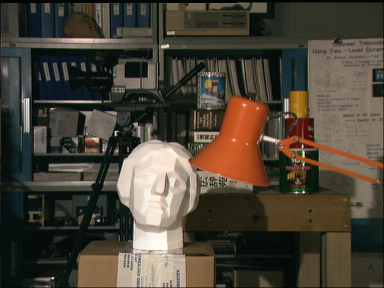
\includegraphics[width=4cm]{../code/dataset/l.png}
                \caption{左目图像}
                \label{lfig}
            \end{minipage}
            \begin{minipage}[t]{0.3\textwidth}
                \centering
                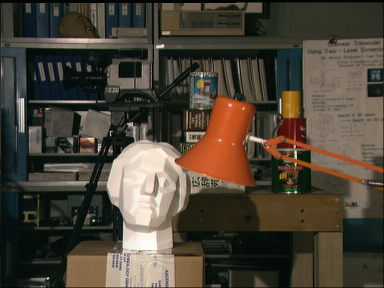
\includegraphics[width=4cm]{../code/dataset/r.png}
                \caption{右目图像}
                \label{rfig}
            \end{minipage}
            \begin{minipage}[t]{0.3\textwidth}
                \centering
                \includegraphics[width=4cm]{../code/result/example_gray.jpg}
                \caption{视差图}
                \label{disfig}
            \end{minipage}
        \end{figure}

    \subsection{将灰度图转化为伪彩色图像}
    为了使生成的图像便于观察,使用opencv的applyMapColor函数将灰度图转化为彩色图像。

    \begin{figure}[htbp]
        \centering
        \begin{minipage}[t]{0.4\textwidth}
            \centering
            \includegraphics[width=5cm]{../code/result/example_gray.jpg}
        \end{minipage}
        \begin{minipage}[t]{0.4\textwidth}
            \centering
            \includegraphics[width=5cm]{../code/result/example_fakergb.jpg}
        \end{minipage}
        \caption{将灰度图映射为伪彩色图像}
    \end{figure}


    \subsection{观察SGBM算法的不同参数对结果的影响}
    SGBM重要参数如下所示:
    \begin{enumerate}
        \item \textbf{MinDisparity},即最小视差,本实验中将其设置为0,因为两个摄像头是前向平行放置,相同的物体在左图中一定比在右图中偏右。如果为了追求更大的双目重合区域而将两个摄像头向内偏转的话,这个参数是需要考虑的。 

        \item \textbf{UniquenessRatio},主要可以防止误匹配,此参数对于最后的匹配结果是有很大的影响。立体匹配中,宁愿区域无法匹配,也不要误匹配。如果有误匹配的话,碰到障碍检测这种应用,就会很麻烦。该参数不能为负值,一般5-15左右的值比较合适,int型。

        \item \textbf{BlockSize},SAD窗口大小,容许范围是[5,255],一般应该在 5x5..21x21 之间,参数必须为奇数值, int型。 

        \item \textbf{NumDisparities},视差窗口,即最大视差值与最小视差值之差,窗口大小必须是 16的整数倍,int型。
    \end{enumerate}

    在SGBM算法的参数中,对视差生成效果影响较大的主要参数是BlockSize、NumDisparities和UniquenessRatio三个,一般只需对这三个参数进行调整,其余参数按默认设置即可。本节将着重观察BlockSize和NumDisparities两个参数对结果的影响。图\ref{bigfig}展示了不同的参数对最终生成的视差图的影响。

    可以看到,较大的BlockSize可以使得生成的视差图更加平滑,而较大的NumDisparities会使画面左侧出现黑色边框,所以使用较小的NumDisparities和较大的BlockSize可以获得比较好的视差图效果。
    \begin{figure}\centering\subfigure[$N_d=16, S_b=7$] {
    \centering
    \includegraphics[width=3.2cm]{../code/result/16_7.png}
}
\subfigure[$N_d=16, S_b=11$] {
    \centering
    \includegraphics[width=3.2cm]{../code/result/16_11.png}
}
\subfigure[$N_d=16, S_b=15$] {
    \centering
    \includegraphics[width=3.2cm]{../code/result/16_15.png}
}
\subfigure[$N_d=16, S_b=19$] {
    \centering
    \includegraphics[width=3.2cm]{../code/result/16_19.png}
}
\subfigure[$N_d=32, S_b=7$] {
    \centering
    \includegraphics[width=3.2cm]{../code/result/32_7.png}
}
\subfigure[$N_d=32, S_b=11$] {
    \centering
    \includegraphics[width=3.2cm]{../code/result/32_11.png}
}
\subfigure[$N_d=32, S_b=15$] {
    \centering
    \includegraphics[width=3.2cm]{../code/result/32_15.png}
}
\subfigure[$N_d=32, S_b=19$] {
    \centering
    \includegraphics[width=3.2cm]{../code/result/32_19.png}
}
\subfigure[$N_d=48, S_b=7$] {
    \centering
    \includegraphics[width=3.2cm]{../code/result/48_7.png}
}
\subfigure[$N_d=48, S_b=11$] {
    \centering
    \includegraphics[width=3.2cm]{../code/result/48_11.png}
}
\subfigure[$N_d=48, S_b=15$] {
    \centering
    \includegraphics[width=3.2cm]{../code/result/48_15.png}
}
\subfigure[$N_d=48, S_b=19$] {
    \centering
    \includegraphics[width=3.2cm]{../code/result/48_19.png}
}
\subfigure[$N_d=64, S_b=7$] {
    \centering
    \includegraphics[width=3.2cm]{../code/result/64_7.png}
}
\subfigure[$N_d=64, S_b=11$] {
    \centering
    \includegraphics[width=3.2cm]{../code/result/64_11.png}
}
\subfigure[$N_d=64, S_b=15$] {
    \centering
    \includegraphics[width=3.2cm]{../code/result/64_15.png}
}
\subfigure[$N_d=64, S_b=19$] {
    \centering
    \includegraphics[width=3.2cm]{../code/result/64_19.png}
}
\subfigure[$N_d=80, S_b=7$] {
    \centering
    \includegraphics[width=3.2cm]{../code/result/80_7.png}
}
\subfigure[$N_d=80, S_b=11$] {
    \centering
    \includegraphics[width=3.2cm]{../code/result/80_11.png}
}
\subfigure[$N_d=80, S_b=15$] {
    \centering
    \includegraphics[width=3.2cm]{../code/result/80_15.png}
}
\subfigure[$N_d=80, S_b=19$] {
    \centering
    \includegraphics[width=3.2cm]{../code/result/80_19.png}
}\caption{不同参数对结果的影响}\label{bigfig}\end{figure}

    \newpage
    \section{附录}
    本实验代码已在Github开源,请访问:\url{https://github.com/Yidadaa/Computer-Vision-Assignment/tree/master/Assignment-2}。
    \begin{lstlisting}[language=Python]import cv2
import os
import numpy as np
from matplotlib import pyplot as plt

class DisparityMap:
    def __init__(self, numDisparities, blockSize):
        self.stereo = cv2.StereoSGBM_create(0, numDisparities, blockSize)

    def computeDsiparity(self, l, r):
        return self.stereo.compute(l, r)

    def saveToFile(self, filename, img):
        cv2.imwrite(filename, img)

    def setParams(self, numDisparities, blockSize):
        self.stereo = cv2.StereoSGBM_create(0, numDisparities, blockSize)

if __name__ == '__main__':
    instance = DisparityMap(16, 15)
    lImage = cv2.imread('./dataset/l.png', 0)
    rImage = cv2.imread('./dataset/r.png', 0)

    result_dir = './result'
    for f in os.listdir(result_dir):
        os.remove(result_dir + '/' + f)

    example_gray = 'result/example_gray.jpg'
    example_fakergb = 'result/example_fakergb.jpg'
    disparity = instance.computeDsiparity(lImage, rImage)
    instance.saveToFile(example_gray, disparity)
    gray = cv2.imread(example_gray)
    fakergb = cv2.applyColorMap(gray, cv2.COLORMAP_JET)
    instance.saveToFile(example_fakergb, fakergb)

    numDisparities = list(range(16, 16 * 6, 16))
    blockSize = list(range(7, 23, 4))
    for n in numDisparities:
        for b in blockSize:
            instance.setParams(n, b)
            disparity = instance.computeDsiparity(lImage, rImage)
            fname = 'result/%s_%s.png' % (n, b)
            instance.saveToFile(fname, disparity)
            disparity = cv2.imread(fname, 0)
            disparity = cv2.applyColorMap(disparity, cv2.COLORMAP_JET)
            instance.saveToFile(fname, disparity)
\end{lstlisting}

    \end{document}